\documentclass[11pt,twoside,a4paper]{article}
% http://www-h.eng.cam.ac.uk/help/tpl/textprocessing/latex_maths+pix/node6.html symboles de math
% http://fr.wikibooks.org/wiki/Programmation_LaTeX Programmation latex (wikibook)
%=========================== En-Tete =================================
%--- Insertion de paquetages (optionnel) ---
\usepackage[french]{babel}   % pour dire que le texte est en fran{\'e}ais
\usepackage{a4}	             % pour la taille   
\usepackage[T1]{fontenc}     % pour les font postscript
\usepackage{epsfig}          % pour gerer les images
%\usepackage{psfig}
\usepackage{float}           % pour le placement des figures
\usepackage{verbatim}

\usepackage{longtable} % pour les tableaux de plusieurs pages

\usepackage[table]{xcolor} % couleur de fond des cellules de tableaux

\usepackage{lastpage}

\usepackage{multicol} % pour {\'e}crire dans certaines zones en colonnes : \begin{multicols}{nb colonnes}...\end{multicols} 

% \usepackage[top=1.5cm, bottom=1.5cm, left=1.5cm, right=1.5cm]{geometry}
% gauche, haut, droite, bas, entete, ente2txt, pied, txt2pied
\usepackage{vmargin}
\setmarginsrb{1.00cm}{1.00cm}{1.00cm}{1.00cm}{15pt}{3pt}{15pt}{15pt}

\usepackage{lscape} % changement orientation page
%\usepackage{frbib} % enlever pour obtenir references en anglais
% --- style de page (pour les en-tete) ---

%% \pagestyle{empty}

% % % en-tete et pieds de page configurables : fancyhdr.sty

% http://www.trustonme.net/didactels/250.html

% http://ww3.ac-poitiers.fr/math/tex/pratique/entete/entete.htm
% http://www.ctan.org/tex-archive/macros/latex/contrib/fancyhdr/fancyhdr.pdf
% \usepackage{fancyhdr}
% \pagestyle{fancy}
% % \newcommand{\chaptermark}[1]{\markboth{#1}{}}
% % \newcommand{\sectionmark}[1]{\markright{\thesection\ #1}}
% \fancyhf{}
% \fancyhead[LE,RO]{\bfseries\thepage}
% \fancyhead[LO]{\bfseries\rightmark}
% \fancyhead[RE]{\bfseries\leftmark}
% \fancyfoot[LE]{\thepage /\pageref{LastPage} \hfill
	% TITLE
% \hfill 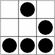
\includegraphics[width=0.5cm]{img/logo_glider.png} }
% \fancyfoot[RO]{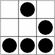
\includegraphics[width=0.5cm]{img/logo_glider.png} \hfill
	% TITLE
% \hfill \thepage /\pageref{LastPage}}
% \renewcommand{\headrulewidth}{0.5pt}
% \renewcommand{\footrulewidth}{0.5pt}
% \addtolength{\headheight}{0.5pt}
% \fancypagestyle{plain}{
	% \fancyhead{}
	% \renewcommand{\headrulewidth}{0pt}
% }

%--- Definitions de nouvelles commandes ---
\newcommand{\N}{\mathbb{N}} % les entiers naturels

%============================= Corps =================================

\begin{document}

\setlength\parindent{0pt} % \noindent for all document

\texttt{http://www.numerama.com/magazine/23363-pas-de-compte-facebook-vous-etes-suspect.html}~\\

\textbf{\LARGE Pas de compte Facebook ? Vous {\^e}tes suspect}~\\

Julien L. -- publi{\'e} le Mardi 07 Ao{\^u}t 2012 {\`a} 19h02 -- post{\'e} dans Soci{\'e}t{\'e} 2.0~\footnote{\texttt{http://www.numerama.com/magazine/societe-20}}~\\

\emph{\small Facebook, R{\'e}seau social, Social, Twitter, {\'E}tats-Unis}~\\

\textbf{Ne pas {\^e}tre inscrit sur Facebook pourrait un jour devenir suspect aux yeux de la population. C'est ce qui ressort d'un article allemand, qui r{\'e}v{\`e}le que des psychologues et des employeurs trouvent anormal de ne pas avoir de compte Facebook. Et de souligner que James Holmes, Mohammed Merah et Anders Breivik n'en avaient pas non plus. Mais c'est oublier qu'une vie sociale active peut aussi se d{\'e}rouler hors de Facebook et m{\^e}me hors du net. }~\\

\begin{minipage}[ht]{0.68\textwidth} 
% ?? ~\footnotemark[footnote] % pour forcer mise en base de page, associ{\'e} {\`a} 'footnotetext'
Quel est le point commun entre James Holmes, Mohammed Merah et Anders Breivik ? Ce sont tous des tueurs en s{\'e}rie qui n'avaient pas de compte Facebook. Un hasard ? Sans doute. Mais il semble que cette particularit{\'e}, relev{\'e}e par la presse allemande~\footnotemark , pourrait {\`a} terme devenir un imp{\'e}ratif social. Car en effet, {\^e}tre absent de Facebook serait le signe, pour certains psychologues et employeurs, d'une potentielle dangerosit{\'e}.~\\

Selon eux, les personnes n'ayant pas de compte Facebook sont suspectes car, d{\`e}s lors, cela signifie qu'elles ont quelque chose {\`a} cacher ou que leur compte a {\'e}t{\'e} supprim{\'e} pour avoir eu un comportement inappropri{\'e} en violation avec les conditions d'utilisation du site. Des entreprises seraient ainsi devenues moins dispos{\'e}es {\`a} engager des individus absents du r{\'e}seau am{\'e}ricain.~\\
\end{minipage} \hfill \begin{minipage}[ht]{0.31\textwidth} 
	
\includegraphics[width=6cm]{img/facebookfaille.jpg}
\end{minipage}
~\footnotetext{\texttt{https://www.tagesspiegel.de/weltspiegel/nach-dem-attentat-von-denver-kein-facebook-profil-kein-job-angebot/6911648-2.html}}

\textbf{Holmes, Merah, Breivik}~\\

James Holmes, qui s'est illustr{\'e} aux {\'E}tats-Unis dans la fusillade d'Aurora o{\`u} 12 personnes ont perdu la vie et 59 autres ont {\'e}t{\'e} bless{\'e}es pendant une s{\'e}ance du film du dernier Batman, {\'e}tait en effet "invisible" sur Internet~\footnote{\texttt{http://www.numerama.com/magazine/23247-l-auteur-de-la-tuerie-d-aurora-invisible-sur-internet.html}}. Il n'{\'e}tait pas inscrit sur Facebook ni sur aucun autre site de r{\'e}seautage social classique sauf celui tr{\`e}s particulier d'AdultFinder. Un cas plut{\^o}t rare pour un Am{\'e}ricain {\^a}g{\'e} de 24 ans et scolaris{\'e}.~\\

Ce point a d'ailleurs interpell{\'e} une chercheuse en m{\'e}decine et sant{\'e} publique. "C'est certainement inhabituel" pour un jeune homme de ne pas {\^e}tre sur les r{\'e}seaux sociaux. "Les donn{\'e}es sugg{\`e}rent que 95 {\`a} 98 \% des gens de l'{\^a}ge de Holmes sont sur les m{\'e}dias sociaux". Ne pas {\^e}tre visible en ligne peut appara{\^i}tre pour certains comme le signe d'une exclusion sociale.~\\

De son c{\^o}t{\'e}, Mohammed Merah, qui a tu{\'e} 7 personnes et bless{\'e} 6 autres {\`a} Toulouse et Montauban, n'{\'e}tait pas particuli{\`e}rement actif en ligne. S'il se connectait effectivement {\`a} Internet, le suivi de son adresse IP montre qu'il n'{\'e}tait pas non plus pr{\'e}sent sur les sites communautaires (Facebook, Twitter, Copains d'avant...). Il {\'e}tait n{\'e}anmoins pr{\'e}sent sur YouTube, dans le but de publier des vid{\'e}os.~\\

Quant {\`a} Anders Breivik, qui est poursuivi pour les attentats de 2011 en Norv{\`e}ge qui ont co{\^u}t{\'e} la vie {\`a} 77 personnes et bless{\'e} 151 autres, il {\'e}tait pr{\'e}sent sur MySpace mais pas sur Facebook. Or, le premier est sur le d{\'e}clin depuis que le second a pris son envol. L{\`a} encore, les psychologues y voient le signe d'un d{\'e}ficit relationnel, puisque ces individus n'ont pas cherch{\'e} {\`a} d{\'e}placer leurs liens d'amiti{\'e} sur Internet.~\\

Autrement dit, ces trois personnes n'auraient pas eu beaucoup d'amis au cours de leur vie, ce qui les aurait dissuad{\'e}s d'aller sur Facebook, craignant de projeter une image n{\'e}gative d'eux-m{\^e}mes. C'est du moins le raisonnement des psychologues et des entrepreneurs cit{\'e}s par le quotidien allemand.~\\

%% \clearpage

\textbf{Des signes de d{\'e}pression relev{\'e}s dans une {\'e}tude}~\\

Une {\'e}tude portant sur la sant{\'e} mentale~\footnote{\texttt{http://pediatrics.aappublications.org/content/early/2011/01/17/peds.2010-1235.abstract}} des jeunes gens alimente cette th{\`e}se. D'apr{\`e}s la recherche men{\'e}e par l'universit{\'e} de Lausanne, en Suisse, le temps pass{\'e} sur Internet aurait un lien avec la d{\'e}pression chez les jeunes, dans une courbe en forme de U. Les adolescents qui montrent le plus de signes de d{\'e}pression seraient {\`a} la fois ceux qui sont le plus souvent actifs sur Internet, et ceux qui au contraire n'y sont jamais.~\\

L'inqui{\'e}tude des psychologues et employeurs signal{\'e}e dans le Tagesspiegel para{\^i}t exag{\'e}r{\'e}e, pour ne pas dire plus. Facebook est peut-{\^e}tre tr{\`e}s populaire, mais il n'est pas l'alpha et l'om{\'e}ga du r{\'e}seautage social sur Internet. Des liens {\'e}taient tiss{\'e}s bien avant le projet de Mark Zuckerberg et seront tiss{\'e}s lorsque Facebook ne sera plus. Tout ne passe pas par ce site, et heureusement.~\\

De nombreux sites communautaires existent par ailleurs, et certains sont tr{\`e}s appr{\'e}ci{\'e}s~\footnote{\texttt{http://www.numerama.com/magazine/18116-tres-populaire-en-france-facebook-ne-domine-pas-encore-partout.html}}. C'est le cas en Allemagne, en Russie, au Japon ou en Chine. Dans ces pays, des r{\'e}seaux sociaux ont su {\'e}merger et {\^e}tre populaire bien avant Facebook. Et cela ne fait pas de ces internautes des personnes en d{\'e}ficit relationnel. Leur r{\'e}seau se trouve tout simplement ailleurs.~\\

Et puis on peut tr{\`e}s bien avoir une vie sociale active sans {\^e}tre sur Internet du tout, m{\^e}me si \c{c}a semble de plus en plus rare.~\\

\clearpage

\texttt{http://www.numerama.com/magazine/23247-l-auteur-de-la-tuerie-d-aurora-invisible-sur-internet.html}~\\

\textbf{\LARGE L'auteur de la tuerie d'Aurora invisible sur Internet}~\\

Guillaume Champeau -- publi{\'e} le Lundi 23 Juillet 2012 {\`a} 16h30 -- post{\'e} dans Soci{\'e}t{\'e} 2.0~\footnote{\texttt{http://www.numerama.com/magazine/societe-20}}~\\

\emph{\small Facebook, R{\'e}seau social, Social, Twitter, {\'E}tats-Unis}~\\

\textbf{Aux {\'E}tats-Unis, la presse se demande pourquoi l'auteur du massacre d'Aurora, {\^a}g{\'e} de 24 ans et en apparence semblable {\`a} tous les jeunes adultes, n'avait aucune pr{\'e}sence visible sur Internet.}~\\

\begin{minipage}[ht]{0.70\textwidth} 
Plus que la conclusion, c'est l'interrogation qui intrigue. Le magazine am{\'e}ricain CNet~\footnotemark s'est interrog{\'e} samedi, comme d'autres journaux sp{\'e}cialis{\'e}s, sur l'absence totale de traces num{\'e}riques de James Eagan Holmes, l'auteur du massacre d'Aurora. Comme si en 2012, tout jeune homme normalement constitu{\'e} devait avoir son nom "Googlable" pour retrouver des informations sur ses centres d'int{\'e}r{\^e}ts, ses amis, ses id{\'e}ologies, etc.~\\

"\emph{Il appara{\^i}t que le suspect Holmes n'est sur aucun r{\'e}seau social -- au moins pas sous son vrai nom}", remarque Cnet. "\emph{Pourtant le portrait qui a {\'e}t{\'e} d{\'e}peint de Holmes n'est pas tr{\`e}s diff{\'e}rent de celui d'un {\'e}tudiant typique, peut-{\^e}tre d{\'e}sabus{\'e} (...) S'il {\'e}tait sur Facebook, nous pourrions peut-{\^e}tre conna{\^i}tre son {\'e}tat d'esprit, ce qu'il a eu {\`a} d{\^i}ner, sur ce qu'il a fait le 4 juillet, ce qui nous donnerait une id{\'e}e de son {\'e}tat mental pr{\'e}alable aux {\'e}v{\`e}nements, mais Holmes est introuvable sur ce r{\'e}seau social, ou sur Twitter}".~\\
\end{minipage} \hfill \begin{minipage}[ht]{0.26\textwidth} 
	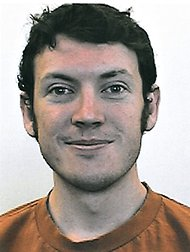
\includegraphics[width=5cm]{img/holmes.jpg}
\end{minipage}
~\footnotetext{\texttt{http://news.cnet.com/8301-1023\_3-57477225-93/the-mystery-of-aurora-suspects-missing-facebook-account/}}

"\emph{Des rapports non confirm{\'e}s vendredi dernier pr{\'e}tendent qu'il pourrait avoir {\'e}t{\'e} sur le site de rencontres AdultFinder.com, pas l'endroit que la plupart choisiraient pour se connecter aux amis, {\`a} la famille, ou au public plus large}".~\\

Interrog{\'e} par le magazine, une chercheuse en m{\'e}decine et sant{\'e} publique reconna{\^i}t que "c'est certainement inhabituel" pour un jeune adulte de ne pas {\^e}tre sur les r{\'e}seaux sociaux. "Les donn{\'e}es sugg{\`e}rent que 95 {\`a} 98 \% des gens de l'{\^a}ge de Holmes sont sur les m{\'e}dias sociaux", affirme-t-il. La Dr. Mega A. Morano cite par ailleurs une {\'e}tude qui montrerait que le temps pass{\'e} sur Internet aurait un lien avec la d{\'e}pression chez les jeunes, dans une courbe en forme de U. Les adolescents qui montrent le plus de signes de d{\'e}pression seraient {\`a} la fois ceux qui sont le plus souvent actifs sur Internet, et ceux qui au contraire n'y sont jamais.~\\ 

En France, Mohammed Merah non plus ne semblait pas avoir eu une pr{\'e}sence en ligne tr{\`e}s importante. Il {\'e}tait bien connect{\'e} sur Internet, comme le montre notamment l'adresse IP qui a servi {\`a} le compromettre sur un site de petites annonces, mais n'avait ni compte Facebook, ni compte Twitter, ou autres Copains D'Avant. Le Toulousain avait n{\'e}anmoins projet{\'e} de diffuser les vid{\'e}os de ses actes de barbarie, et en a {\'e}t{\'e} emp{\^e}ch{\'e} par une limitation technique de YouTube, comme il l'a expliqu{\'e} {\`a} la DCRI dans une discussion diffus{\'e}e par Lib{\'e}ration :~\\

\begin{minipage}[t]{2cm} 
	~\\
\end{minipage} \hfill \begin{minipage}[t]{12cm} 
	\footnotesize %% \small 
    MOHAMED: {\'E}coute je l'ai envoy{\'e}e {\`a}, {\`a} mes alli{\'e}s qui vont la, qui vont la, la, la faire para{\^i}tre sur le net, heu, quand eux ils auront d{\'e}cid{\'e}, t'as vu. Heu, apr{\`e}s vous dire quand pr{\'e}cis{\'e}ment, je saurais vous dire, je l'ai envoy{\'e} et heu, voil{\`a}. Parce que j'ai essay{\'e} de la mettre sur internet mais comme \textbf{c'est une vid{\'e}o qui dure 25 minutes, YOUTUBE l'a refus{\'e} et il a demand{\'e} une vid{\'e}o de 15 minutes}. Je comptais la modifier tout {\`a} l'heure pour la mettre sur le net.
\end{minipage} \hfill \begin{minipage}[t]{2cm} 
	~\\
\end{minipage} ~\\ ~\\

Les deux tueurs avaient le m{\^e}me {\^a}ge (23 ans pour Merah, 24 pour Holmes). -- De son c{\^o}t{\'e}, le New-York Times a publi{\'e} vendredi une enqu{\^e}te, dans laquelle il indique que Holmes aurait "\emph{pass{\'e} beaucoup de temps sur son ordinateur}" dans le laboratoire de son universit{\'e}, et qu'il "\emph{participait souvent {\`a} des jeux de r{\^o}le~\footnote{\texttt{http://www.ludocortex.fr/oniros-initiation-au-jeu-de-role-multisim,fr,4,onirosinitiation.cfm}} en ligne}". De quoi relancer une nouvelle fois la pol{\'e}mique sur les liens entre tueurs fous et jeux vid{\'e}o~\footnote{\texttt{http://www.numerama.com/magazine/22997-natacha-polony-fait-un-lien-direct-entre-merah-et-les-jeux-video.html}}. %% ~\\

\clearpage

\texttt{http://www.numerama.com/magazine/24534-adam-lanza-encore-un-tueur-de-masse-sans-page-facebook.html}~\\

\begin{minipage}[ht]{0.70\textwidth} 
	\textbf{\LARGE Adam Lanza, encore un tueur de masse sans page Facebook}~\\
	
	Guillaume Champeau -- publi{\'e} le Lundi 17 D{\'e}cembre 2012 {\`a} 09h36 -- post{\'e} dans Soci{\'e}t{\'e} 2.0~\footnotemark~\\

	\emph{\small Facebook, R{\'e}seau social}~\\
\end{minipage} \hfill \begin{minipage}[ht]{0.28\textwidth} 
	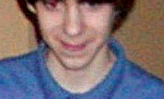
\includegraphics[width=1.00\textwidth]{img/lanza.png}
\end{minipage}
\footnotetext{\texttt{http://www.numerama.com/magazine/societe-20}}


\textbf{Apr{\`e}s Breivik, Merah et Holmes, l'auteur de la tuerie de Newton Adam Lanza perp{\'e}tue la caract{\'e}ristique des tueurs de masse de l'{\'e}poque r{\'e}cente, de ne pas avoir de page Facebook. Plus qu'une co{\"i}ncidence, cela devient une r{\`e}gle. }~\\

Force est de reconna{\^i}tre que cela devient plus qu'une co{\"i}ncidence. Apr{\`e}s l'auteur de la tuerie de Norv{\`e}ge Anders Behring Breivik, apr{\`e}s l'auteur de la tuerie de Toulouse Mohammed Mehah \emph{[Merah, ...]}, apr{\`e}s l'auteur de la tuerie du cin{\'e}ma d'Aurora James Holmes, voici qu'Adam Lanza partage lui aussi le m{\^e}me trait commun. Comme ces derniers, l'auteur de la tuerie de Newton semble avoir parmi ses caract{\'e}ristiques de \texttt{ne pas {\^e}tre inscrit sur Facebook}~\footnotemark  alors qu'il est {\`a} un {\^a}ge, 20 ans, o{\`u} plus des trois quarts des Am{\'e}ricains sont inscrits sur le premier r{\'e}seau social du monde. ~\\
\footnotetext{\texttt{http://www.lexpress.fr/actualite/monde/amerique/fusillade-de-newtown-que-sait-on-d-adam-lanza-le-tueur-du-connecticut\_1199623.html}}

\begin{minipage}[ht]{0.70\textwidth} 
	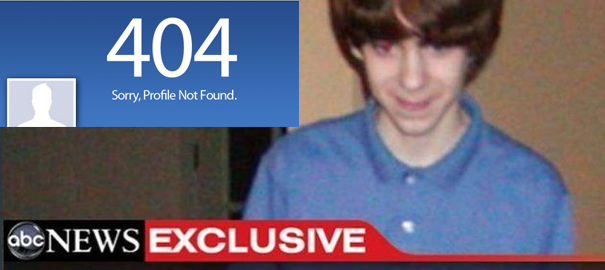
\includegraphics[width=1.00\textwidth]{img/facebook-adamlanza.png}
\end{minipage} \hfill \begin{minipage}[ht]{0.28\textwidth} 
	Apr{\`e}s le massacre commis par James Holmes lors de l'avant-premi{\`e}re de Batman, aux Etats-Unis, la presse allemande avait d{\'e}j{\`a} remarqu{\'e} ce trait sp{\'e}cifique chez une s{\'e}rie d'auteurs de crimes massifs. Aucun d'entre eux n'{\'e}taient inscrits sur Facebook, alors que selon une chercheuse interrog{\'e}e {\`a} l'{\'e}poque, "\emph{les donn{\'e}es sugg{\`e}rent que 95 {\`a} 98 \% des gens de l'{\^a}ge de Holmes sont sur les m{\'e}dias sociaux}". ~\\
\end{minipage}

Forc{\'e}ment, le fait qu'Adam Lanza lui non plus n'{\'e}tait pas inscrit sur le r{\'e}seau social va renforcer l'id{\'e}e de \texttt{devenir suspect si l'on a pas de page Facebook~\footnotemark}. ~\\
\footnotetext{\texttt{http://www.numerama.com/magazine/23363-pas-de-compte-facebook-vous-etes-suspect.html}}

Car aujourd'hui, ne pas avoir de compte Facebook est vu comme un sympt{\^o}me de non-int{\'e}gration sociale, qui peut elle-m{\^e}me provoquer les pulsions meurtri{\`e}res. Breivik, Holmes et Merah n'avaient jamais eu beaucoup d'amis "dans la vraie vie", et n'ont pas ressenti le besoin, l'envie ou la n{\'e}cessit{\'e} de s'inscrire sur un site Internet comme Facebook o{\`u} tout est organis{\'e} autour des amis qu'ils n'ont pas. C'est la m{\^e}me chose pour Adam Lanza, qui est d{\'e}crit comme un un adolescent "\texttt{l{\'e}g{\`e}rement autiste~\footnotemark}", tr{\`e}s intelligent mais "souvent tout seul", qui n'avait pas ou tr{\`e}s peu d'amis. ~\\
\footnotetext{\texttt{http://www.europe1.fr/International/Newtown-un-tueur-un-peu-different-et-perturbe-1348627/}}

"\emph{Les tueurs de masse sont souvent des gens individualistes, repli{\'e}s sur eux-m{\^e}mes, introvertis, qui sont souvent en {\'e}chec relationnel, en {\'e}chec social, et qui parall{\`e}lement ont des traits parano{\"i}aques}", \texttt{expliquait sur iT{\'e}l{\'e}~\footnotemark} le psychiatre et criminologue Roland Coutanceau. "\emph{Ils ressentent les autres comme rejetant, ils se sentent mal aim{\'e}s, mal compris, d'o{\`u} au fond la naissance de cette rage destructrice qui va soutenir ce passage {\`a} l'acte hors normes}". ~\\
\footnotetext{\texttt{http://www.itele.fr/video/profil-du-tueur-de-newtown-les-tueurs-de-masse-ne-sont-pas-des-fous}}

\clearpage

\texttt{http://www.europe1.fr/International/Newtown-un-tueur-un-peu-different-et-perturbe-1348627/}~\\

\textbf{\LARGE Newtown : un tueur "un peu diff{\'e}rent" et "perturb{\'e}"}~\\

Par \textbf{W, avec agences et G{\'e}raldine Woessner {\`a} Newtown}~\\

\emph{Publi{\'e} le 15 d{\'e}cembre 2012 {\`a} 09h10 -- Mis {\`a} jour le 15 d{\'e}cembre 2012 {\`a} 14h03}~\\

\begin{minipage}[ht]{0.42\textwidth}
	\begin{center}
		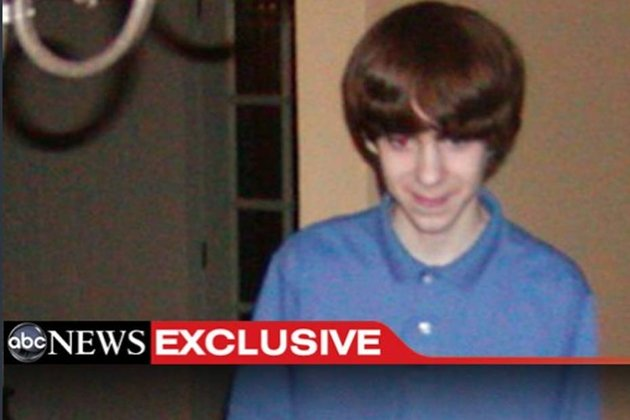
\includegraphics[width=1.00\textwidth]{img/La-premiere-photo-d-Adam-Lanza-a-ete-diffusee-par-ABC-News-Le-cliche-date-de-2005-il-avait-alors-13-ans.jpg}
		\emph{\small La premi{\`e}re photo d'Adam Lanza a {\'e}t{\'e} diffus{\'e}e par ABC News. Le clich{\'e} date de 2005, il avait alors 13 ans. \copyright CAPTURE ABC News}~\\
	\end{center}
\end{minipage} \hfill \begin{minipage}[ht]{0.55\textwidth} 
	\textbf{PORTRAIT -- Le jeune homme avait lui-m{\^e}me {\'e}t{\'e} scolaris{\'e} dans l'{\'e}tablissement o{\`u} il a fait feu. }~\\

	Qui est Adam Lanza ? C'est ce que cherchent {\`a} savoir tous les m{\'e}dias am{\'e}ricains quelques heures apr{\`e}s \texttt{la tuerie {\`a} l'{\'e}cole Sandy Hook de Newtown~\footnotemark}, dans le Connecticut. Pour l'heure, la police n'a pas encore publiquement confirm{\'e} que le jeune homme de 20 ans {\'e}tait le tueur, tout indique cependant qu'il est bien l'auteur du massacre \texttt{qui a co{\^u}t{\'e} la vie {\`a} 20 enfants et six adultes~\footnotemark}. Plusieurs t{\'e}moignages donnent un {\'e}clairage sur sa personnalit{\'e}. ~\\
	
	\textbf{Un jeune homme "l{\'e}g{\`e}rement autiste"}~\\
\end{minipage}~\\~\\
\footnotetext{\texttt{http://www.europe1.fr/International/Fusillade-de-Newtown-ce-qui-s-est-passe-1348523/}}
\footnotetext{\texttt{http://www.europe1.fr/International/USA-fusillade-meurtriere-dans-une-ecole-1348333/}}

%% {\small
	Outre Atlantique, plusieurs connaissances du tueur pr{\'e}sum{\'e} font {\'e}tat d'un jeune homme ayant "des probl{\`e}mes psychologiques" et un comportement "perturb{\'e}" voire "l{\'e}g{\`e}rement autiste" m{\^e}me si on ignore si un diagnostic avait {\'e}t{\'e} pos{\'e}. Au micro d'Europe1, la m{\`e}re d'un camarade d'Adam a d{\'e}crit un gar\c{c}on "tr{\`e}s r{\'e}serv{\'e}, maigre et le visage p{\^a}le", "un gothique" d'apr{\`e}s son fils, "souvent tout seul". --- Adam n'{\'e}tait "de toute {\'e}vidence pas bien", a confirm{\'e} un proche de la famille Lanza cit{\'e} par ABC News. Sur la cha{\^i}ne, des amis de la famille ont aussi d{\'e}crit un jeune homme "troubl{\'e}" et une m{\`e}re "rigide". "Adam {\'e}tait un peu diff{\'e}rent, comme opprim{\'e}", a confi{\'e} une proche de la famille toujours sur ABC News. ~\\
	
	\textbf{Press{\'e} de r{\'e}ussir {\`a} l'{\'e}cole}~\\
	
	Deux anciens camarades de classe d'Adam Lanza disent, eux, se souvenir d'un gar\c{c}on timide et intelligent. --- Au lyc{\'e}e de Newtown, il se distinguait des autres {\'e}l{\`e}ves par son style vestimentaire plus strict, avec souvent des chemises boutonn{\'e}es jusqu'au col, raconte Tim Arnone, qui l'a connu {\`a} l'{\'e}cole Sandy Hook. ~\\
	
	Ensemble, ils faisaient partie du club audiovisuel du lyc{\'e}e et passaient de longs moments {\`a} jouer aux jeux vid{\'e}o dans la salle de t{\'e}l{\'e}vision de l'{\'e}tablissement. "C'{\'e}tait assur{\'e}ment le club le plus ringard de l'{\'e}cole. (...) On avait notre petit coin {\`a} nous dans la pi{\`e}ce", dit Tim Arnone, 20 ans. --- Selon ce dernier, les parents d'Adam Lanza, en particulier sa m{\`e}re, {\'e}taient extr{\^e}mement soucieux de la r{\'e}ussite scolaire de leur fils. "Elle le poussait vraiment fort {\`a} {\^e}tre plus intelligent et {\`a} travailler plus dur {\`a} l'{\'e}cole", se souvient-il. ~\\
	
	\textbf{Intelligent mais esseul{\'e}}~\\
	
	Un autre ancien camarade de classe ayant requis l'anonymat d{\'e}crit Adam Lanza comme quelqu'un d'intelligent mais sans beaucoup d'amis. Il dit avoir rencontr{\'e} Adam Lanza lorsqu'ils ont int{\'e}gr{\'e} ensemble l'antenne locale des scouts. A l'{\'e}poque, dit-il, Adam Lanza adorait ce qui venait du Japon, il collectionnait les cartes Pokemon et jouait sur sa console PlayStation {\`a} Dynasty Warriors, un jeu de combat avec armes {\`a} feu sorti dans les ann{\'e}es 1990. ~\\
	
	"C'{\'e}tait un gar\c{c}on tr{\`e}s calme", dit cet ancien camarade. "Je me souviens que j'{\'e}tais son seul ami en primaire. Il a toujours {\'e}t{\'e} un enfant vraiment gentil, tr{\`e}s poli. ~\\
	
	\textbf{Il s'exer\c{c}ait au tir avec sa m{\`e}re, collectionneuse d'armes}~\\
	
	Nancy Lanza et son mari Peter Lanza ont divorc{\'e} en 2008, selon les documents officiels. Selon Dan Holmes, un paysagiste de Newtown ayant install{\'e} la semaine derni{\`e}re des d{\'e}corations de No{\"e}l dans le jardin de Nancy Lanza, cette derni{\`e}re {\'e}tait "tr{\`e}s charmante" et collectionnait les armes {\`a} feu. "Elle disait qu'elle allait souvent s'exercer au tir avec ses enfants", dit Dan Holmes. ~\\
	
	\textbf{"Pr{\'e}m{\'e}ditation, r{\'e}flexion et organisation" ?}~\\
	
	"Ce qu'il faut souligner au sujet des individus comme Adam Lanza c'est qu'il ne s'est pas r{\'e}veill{\'e} soudainement un matin en d{\'e}cidant d'{\^e}tre violent", a soulign{\'e} un ancien profiler du FBI, Mary Ellen O'Toole. "Ce genre d'actes impliquent pr{\'e}m{\'e}ditation, r{\'e}flexion et organisation." ~\\
%% } % \small

\dotfill

\texttt{http://www.lexpress.fr/actualite/monde/amerique/fusillade-de-newtown-que-sait-on-d-adam-lanza-le-tueur-du-connecticut\_1199623.html}~\\

\textbf{\large Fusillade de Newtown: qui {\'e}tait Adam Lanza, le tueur du Connecticut?}~\\

\emph{\small Par LEXPRESS.fr, publi{\'e} le 15/12/2012 {\`a} 09:40, mis {\`a} jour {\`a} 20:00}~\\

\textbf{Il a tu{\'e} vingt enfants et six adultes, dont sa m{\`e}re. Qui {\'e}tait Adam Lanza, {\^a}g{\'e} d'{\`a} peine 20 ans, pour commettre une telle atrocit{\'e}?}~\\ 

Il a tu{\'e} vingt enfants et six adultes, dont sa m{\`e}re. Qui {\'e}tait Adam Lanza, {\^a}g{\'e} d'{\`a} peine 20 ans, pour commettre une telle atrocit{\'e}, plongeant une nouvelle fois les Etats-Unis dans le deuil? Pour l'heure, les informations sont {\'e}parses sur l'identit{\'e} et la personnalit{\'e} du jeune tueur du Connecticut, soup\c{c}onn{\'e} d'avoir froidement abattu 26 personnes dont 20 enfants vendredi dans l'{\'e}cole primaire de \texttt{Sandy Hook~\footnote{\texttt{http://www.lexpress.fr/infos/pers/sandy-hook.html}}}, {\`a} Newtown, avant de se suicider. ~\\  

\textbf{\emph{> > > Lire aussi: le d{\'e}roul{\'e} des faits et les zones d'ombres~\footnote{\texttt{http://www.lexpress.fr/actualite/monde/fusillade-de-newtown-le-deroule-des-faits-et-les-zones-d-ombres\_1199696.html}}}} ~\\

Selon un premier portrait dress{\'e} par le \texttt{\emph{New York Times}~\footnote{\texttt{http://www.nytimes.com/2012/12/15/nyregion/adam-lanza-an-enigma-who-is-now-identified-as-a-mass-killer.html}}}, Adam Lanza n'{\'e}tait pas connu des services de police et faisait tout pour rester discret. Sur l'album souvenir de sa classe en 2010, il n'appara{\^i}t pas: trop timide pour {\^e}tre photographi{\'e}. "Si vous le regardiez, il ne semblait ressentir aucune {\'e}motion", a confi{\'e} au New York Timesun de ceux qui le c{\^o}toyaient alors. ~\\  

\textbf{\emph{> > Retrouvez les derni{\`e}res informations sur la fusillade~\footnote{\texttt{http://www.lexpress.fr/actualite/monde/amerique/en-direct-fusillade-de-newtown-les-etats-unis-sous-le-choc-apres-la-mort-de-20-enfants\_1199617.html}}}} ~\\

\textbf{Un gar\c{c}on tr{\`e}s intelligent, "presque autiste"}~\\

Tr{\`e}s intelligent, introverti et nerveux, selon le \emph{New York Times}, Adam Lanza avait {\'e}t{\'e} distingu{\'e} en 2007, recevant des "high honors" r{\'e}serv{\'e}s aux bons {\'e}l{\`e}ves. Il a aussi {\'e}t{\'e} d{\'e}crit comme "presque autiste" par son fr{\`e}re, Ryan Lanza, qu'il n'avait pas vu depuis 2010, et dans un premier temps accus{\'e} de la tuerie parce que ses papiers d'identit{\'e} ont {\'e}t{\'e} retrouv{\'e}s sur le corps de son fr{\`e}re. Un diagnostic partag{\'e} par certains des camarade de classe d'Adam, {\`a} qui on aurait dit que ce dernier souffrait du syndrome d'Asperger, un trouble du spectre autistique qui se caract{\'e}rise par des difficult{\'e}s dans les interactions sociales. ~\\ 

Socialement, Adam Lanza {\'e}tait donc un {\^e}tre {\'e}trange. A l'inverse de la plupart des jeunes de sa g{\'e}n{\'e}ration, il n'avait apparemment pas de page Facebook. "C'{\'e}tait un enfant socialement bizarre", a confi{\'e} une voisine, Beth Israel. "Il {\'e}tait solitaire. Je ne sais pas qui {\'e}taient ses amis". Sa fille Alex a d{\'e}crit le jeune homme comme "incapable de rester en place" et "mal {\`a} l'aise si vous le regardiez".  ~\\

Il faisait partie du "club le plus ringard de l'{\'e}cole", a de son c{\^o}t{\'e} racont{\'e} Tim Arnone {\`a} l'agence Reuters, un ancien camarade de l'{\'e}cole Sandy Hook, {\`a} Newton, o{\`u} Adam a fait son primaire, et avec qui il aurait jou{\'e} {\`a} des jeux vid{\'e}os. Une autre camarade cit{\'e}e par le quotidien am{\'e}ricain s'est rappel{\'e}e de l'obsession d'Adam pour les extraterrestres et son go{\^u}t de "faire exploser des trucs" lorsqu'il {\'e}tait au coll{\`e}ge. A l'{\'e}poque, Adam Lanza adorait tout ce qui venait du Japon: il collectionnait les cartes Pok{\'e}mon et jouait sur sa console PlayStation {\`a} Dynasty Warriors, un jeu de combat avec armes {\`a} feu sorti dans les ann{\'e}es 1990. Mais selon un ancien camarade, c'{\'e}tait un gar\c{c}on tr{\`e}s calme: "Je me souviens que j'{\'e}tais son seul ami en primaire. Il a toujours {\'e}t{\'e} un enfant vraiment gentil, tr{\`e}s poli. " ~\\ 

Pas int{\'e}gr{\'e} {\`a} l'{\'e}cole, il ne l'{\'e}tait pas non plus dans la communaut{\'e} tranquille, de Newtown, 27 000 habitants, mod{\`e}le m{\^e}me de la petite ville am{\'e}ricaine sans histoires. C'est l{\`a} que le r{\'e}alisateur Elia Kazan avait tourn{\'e} "Les Visiteurs" en 1972, un drame sur fond de traumatisme li{\'e} {\`a} la guerre du Vietnam et de vengeance.  ~\\

\emph{[La fusillade en images]}~\\

\textbf{Un divorce parental mal v{\'e}cu}~\\

Adam Lanza n'a a priori pas eu une enfance malheureuse. Peter, son p{\`e}re, annonc{\'e} mort dans un premier temps (mais en r{\'e}alit{\'e} en vie), occupe un poste {\`a} responsabilit{\'e} chez General Electric. Remari{\'e} depuis peu, il aurait peu de contacts avec son fils. Son fr{\`e}re Ryan, 24 ans, est conseiller fiscal chez Ernst \& Young. ~\\

Ses parents divorcent en 2008, et Adam reste vivre chez sa m{\`e}re, dans une jolie maison bourgeoise de Newtown. Selon un ancien voisin, Ryan Kraft, interrog{\'e} par le Washington Post, les fr{\`e}res Lanza auraient souffert du divorce de leurs parents. Adam piquait aussi des col{\`e}res, selon ce voisin, "beaucoup plus que les enfants ordinaires". ~\\

Quant {\`a} Sandy, la m{\`e}re assassin{\'e}e, les voisins la d{\'e}crivent dans le New Yok Times comme tr{\`e}s impliqu{\'e}e dans la vie de ses enfants. "Elle le poussait vraiment fort {\`a} {\^e}tre plus intelligent et {\`a} travailler plus dur {\`a} l'{\'e}cole" se souvient notamment Tim Arnone. Contrairement {\`a} ce qui a {\'e}t{\'e} dit dans un premier temps, Nancy Lanza ne travaillait a priori plus dans l'{\'e}cole de Sandy Hook. Elle a {\'e}t{\'e} tu{\'e}e chez elle, avant que son fils ne se rende dans l'{\'e}tablissement primaire. ~\\

\textbf{Une m{\`e}re passionn{\'e}e d'armes {\`a} feu}~\\

Passionn{\'e}e d'armes {\`a} feu, selon Reuters, Nancy Lanza pratiquait r{\'e}guli{\`e}rement le tir avec ses enfants. Elle poss{\'e}dait des pistolet Sig Sauer et Glock, ainsi qu'un Bushmaster.223, version civile du fusil M16 de l'arm{\'e}e am{\'e}ricaine. Retrouv{\'e}es vendredi sur la sc{\`e}ne du crime..  ~\\

\clearpage

\texttt{http://www.linformaticien.com/actualites/id/27443/ces-tueurs-qui-n-ont-pas-de-page-facebook.aspx}~\\

\textbf{\LARGE Ces tueurs qui n'ont pas de page Facebook}~\\

\emph{par Emilien Ercolani, le 17 d{\'e}cembre 2012 12:18}~\\

\textbf{C'est un constat : les tueurs <<de masse>> notamment aux Etats-Unis ne poss{\`e}dent pas de page Facebook. Adam Lanza, {\`a} l'origine du massacre de Newtown, en fournit un nouvel exemple. M{\^e}me si cette sp{\'e}cificit{\'e} n'est que l'un des indices du caract{\`e}re individualiste et introverti de ces tueurs. }~\\ 

Le nom de l'auteur de la tuerie de Newtown vient s'ajouter {\`a} la triste liste des tueurs de ces derni{\`e}res ann{\'e}es non-inscrits sur le r{\'e}seau social le plus utilis{\'e} au monde, Facebook. Apr{\`e}s Anders Behring Breivik en Norv{\`e}ge, le Fran\c{c}ais Mohammed Mehah {\`a} Toulouse, ou encore l'Am{\'e}ricain James Holmes, auteur du massacre dans le cin{\'e}ma d'Aurora, Adam Lanza est un {\'e}ni{\`e}me tueur <<\emph{d{\'e}connect{\'e}}>>. ~\\ 

C'est un constat dress{\'e} par plusieurs psychiatres interrog{\'e}s sur les tueries de ce genre depuis quelques ann{\'e}es ; mais c'est aussi un trait commun qui semble <<\emph{normal}>> quand on se penche sur la personnalit{\'e} de ces personnes. On parle d'eux comme des <<\emph{individualistes}>>, <<\emph{introvertis}>>, des personnes qui sont <<\emph{{\`a} la limite de l'autisme}>>, des <<\emph{mal aim{\'e}s}>>, <<\emph{mal compris}>> au caract{\`e}re <<\emph{parano{\"i}aque}>>. Et la plupart du temps, ils n'ont pas ou tr{\`e}s peu d'amis, et donc absolument aucune envie et aucun besoin de s'inscrire sur Facebook ou un autre r{\'e}seau o{\`u} les relations sociales sont au c\oe ur du syst{\`e}me. ~\\

\textbf{Ni Facebook, ni Yearbook} ~\\

M{\^e}me les m{\'e}dias semblent assez atterr{\'e}s qu'un jeune am{\'e}ricain de 20 ans, r{\'e}sidant dans une lointaine banlieue cossue de New York, ne poss{\'e}dait pas de page Facebook. <<\emph{{\`A} Newtown, Adam Lanza, un tueur coup{\'e} du monde}>>, titre Lib{\'e}ration quand Le Monde est carr{\'e}ment {\'e}pat{\'e} : <<\emph{Newtown : le tueur n'avait m{\^e}me pas de page Facebook}>>. Un <<\emph{m{\^e}me pas}>> qui en dit long... ~\\

Pour Adam Lanza, cette envie de rester {\'e}loign{\'e} des autres semble plus profonde encore, lui qui {\'e}tait <<\emph{camera shy}>> (timide devant les cam{\'e}ras) raconte-on, qui refusait d'appara{\^i}tre dans le Yearbook, le trombinoscope de fin d'ann{\'e}e, et qui portait sur lui les papiers de son fr{\`e}re Ryan Lanza comme pour dire qu'il n'{\'e}tait pas responsable, jusqu'au bout. ~\\

Attention toutefois {\`a} ne pas tomber dans la b{\^e}tise de l'information brute : les personnes qui n'ont pas de page Facebook seraient des tueurs en s{\'e}rie potentiels ! Peut-{\^e}tre des internautes particuli{\`e}rement soucieux de leur vie priv{\'e}e, tout simplement. ~\\

Notons que plusieurs pages Facebook <<Adam Lanza>> ont r{\'e}cemment {\'e}t{\'e} ouvertes, tr{\`e}s peu fr{\'e}quent{\'e}es pour la plupart. En revanche, l'une d'elles a attir{\'e} notre attention : intitul{\'e}e <<Adam Lanza>>, pr{\'e}sent{\'e} comme un <<reporter t{\'e}l{\'e}>>, la page est vou{\'e}e {\`a} recueillir les t{\'e}moignages <<\emph{des sentiments de haine que vous ressentez suite {\`a} cette horrible trag{\'e}die}>>... ~\\

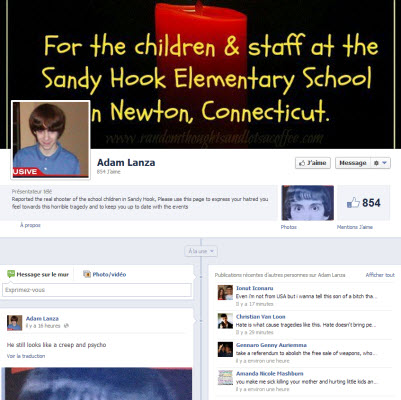
\includegraphics[width=0.30\textwidth]{img/Falanza.jpg}

\clearpage

\texttt{http://www.rue89.com/2012/12/15/le-tueur-de-newton-20-ans-na-pas-facebook-suspect-bravo-france-info-237836}~\\

\textbf{On n'<<aime>> pas} --- 15/12/2012 {\`a} 10h55~\\

\textbf{\LARGE Le tueur de Newtown, 20 ans, n'a pas Facebook, grave ? Bravo France Info}

{\small \textbf{Blandine Grosjean} | \emph{Redchef adj} Rue89}~\\


\emph{Mis {\`a} jour le samedi 15 d{\'e}cembre 2012 {\`a} 11h50}~\\
\emph{Le mot "suspect" est remplac{\'e} par "important" dans la citation (de m{\'e}moire) de France Info.}~\\

Un samedi matin dans ma salle de bains, France Info {\`a} fond pour couvrir le bruit de la douche, et dans la t{\^e}te, mon programme d'une journ{\'e}e o{\`u} je ne vais, enfin, pas travailler. La tuerie de Newtown, une analyse int{\'e}ressante de \texttt{Fabienne Sintes~\footnotemark}, correspondante permanente aux Etat-Unis de la station, sur le d{\'e}bat qui reprend de plus belle entre conservateurs et d{\'e}mocrates {\`a} propos du port d'arme. ~\\
\footnotetext{\texttt{http://radiofrance-blogs.com/fabienne-sintes/}}

Suit un entretien entre la journaliste qui assure la matinale {\`a} Paris et un psychiatre expert aupr{\`e}s des cours d'assises, le professeur Roland Coutanceau, par ailleurs criminologue, pr{\'e}sident de la Ligue fran\c{c}aise de la sant{\'e} mentale. ~\\

\textbf{Il faut bien tenir le <<sp{\'e}cial tuerie>>}~\\

C'est toujours risqu{\'e} de donner un avis <<scientifique>> sur une affaire dont on ne sait encore pas grand-chose, un jeune homme que personne ne conna{\^i}t et qu'il n'a ni vu ni entendu...Passons, il faut du contenu pour tenir le <<sp{\'e}cial tuerie>>. Il parle des traits r{\'e}currents chez les tueurs de masse, l'isolement, la parano, etc. ~\\

\begin{minipage}[h]{0.75\textwidth}
	La journaliste lui pose alors cette question (de m{\'e}moire) : ~\\~\\
	\begin{minipage}[h]{0.10\textwidth} ~\\ \end{minipage} \hfill \begin{minipage}[h]{0.70\textwidth}
		<<\emph{Mais est-ce que le fait de ne pas avoir de page Facebook {\`a} 20 ans est quelque chose d'important ?>>}
	\end{minipage} \hfill \begin{minipage}[h]{0.15\textwidth} ~\\ \end{minipage} ~\\~\\
	Depuis vendredi soir, toute la presse s'enflamme sur le \texttt{<<fail>>~\footnotemark} (bourde) de journalistes am{\'e}ricains qui ont cru trouver le profil du tueur, sur le r{\'e}seau social et ont trouv{\'e} celui de son fr{\`e}re, un travailleur tranquille. ~\\
\end{minipage} \hfill \begin{minipage}[h]{0.25\textwidth}
	\begin{center}
		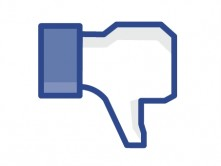
\includegraphics[width=1.00\textwidth]{img/pouce_dislike_facebook.jpg}~\\
		\emph{Le pouce <<J'aime>> de Facebook, {\`a} l'envers}
	\end{center}
\end{minipage}~\\~\\

\footnotetext{\texttt{http://www.rue89.com/2012/12/14/la-presse-americaine-cherche-le-facebook-du-tueur-et-semmele-les-pinceaux-237832}}

\textbf{{\`A} 20 ans, si tu n'as pas de profil Facebook...}~\\

Adam n'aurait pas de profil Facebook. A 20 ans. C'est trop bizarre. Cela confirmerait qu'il {\'e}tait <<isol{\'e}>>, la caract{\'e}ristique des psychopathes, tueurs en s{\'e}rie. A 20 ans, si tu n'as pas de Facebook, c'est que tu n'es pas vraiment {\'e}panoui, tu n'as pas d'amis, pas de vie sociale, tu es anormal, asocial. Voil{\`a}, si tu n'as pas Facebook, \texttt{tu es un mec louche~\footnotemark}. ~\\
\footnotetext{\texttt{http://www.rue89.com/2012/08/08/je-nai-pas-facebook-et-je-ne-suis-pas-un-mec-louche-234476}}

Ma fille de 17 ans a entendu cette question et \c{c}a l'a {\'e}nerv{\'e}e. Elle \texttt{s'est retir{\'e}e de Facebook~\footnotemark} il y a deux ans parce qu'elle trouvait que cela pourrissait ses relations amicales, lui faisait perdre un temps pr{\'e}cieux qu'elle pr{\'e}f{\'e}rait consacrer {\`a} ses amis justement et {\`a} ses passions.
\footnotetext{\texttt{http://www.rue89.com/2012/02/25/pourquoi-et-surtout-comment-ils-ont-quitte-facebook-229643}}

J'ai <<tweet{\'e}>> alors que je m'{\'e}tais promis de me tenir {\'e}loign{\'e}e ce samedi de tous les instruments qui m'encha{\^i}nent au travail. Et j'ai au moins eu la satisfaction de ne pas me sentir isol{\'e}e. ~\\

\clearpage

\texttt{http://www.rue89.com/2012/08/08/je-nai-pas-facebook-et-je-ne-suis-pas-un-mec-louche-234476}~\\

\textbf{T{\'e}moignage} --- 08/08/2012 {\`a} 13h16\\

\textbf{\LARGE Je n'ai pas Facebook et je ne suis pas un mec louche}~\\

{\small \textbf{Sammy~\footnote{\texttt{http://riverains.rue89.com/sammy-0}}} | \emph{Avocat} }~\\

\begin{minipage}[h]{0.42\textwidth}
	\begin{center}
		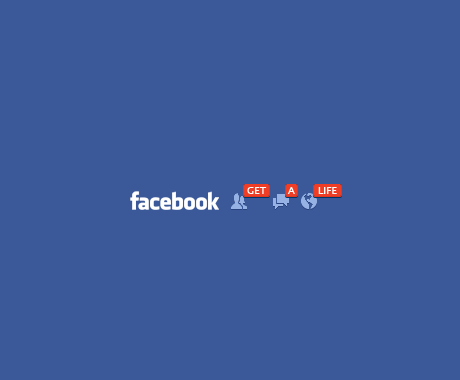
\includegraphics[width=1.00\textwidth]{img/1211-facebook-get-a-life_0.png}~\\
		\emph{<<Get a life>> (va t'acheter une vie), le logo Facebook d{\'e}tourn{\'e} (Boltron/Flickr/CC)~\footnotemark}
	\end{center}
\end{minipage} \hfill \begin{minipage}[h]{0.55\textwidth}
	Pour certains employeurs et psychologues, un jeune n'ayant pas Facebook serait quelqu'un de suspect. C'est ce que j'ai lu dans un article paru dans le \texttt{Daily Mail~\footnotemark}, repris en fran\c{c}ais par Les Inrocks ou encore \texttt{Numerama~\footnotemark}. Il relate les conclusions d'une {\'e}tude men{\'e}e par un magazine allemand, <<Der Tagesspiegel>>. ~\\
	
	L'{\'e}tude va jusqu'{\`a} faire un grossier amalgame entre celui qui ne poss{\'e}derait pas de compte Facebook et certains criminels, comme James Holmes, le tueur d'Aurora, ou encore Mohamed Merah. ~\\

	Pire encore, un autre parall{\`e}le est fait entre le fait d'avoir Facebook et d'entretenir une vie sociale active. ~\\
	
	\textbf{J'{\'e}tais devenu un v{\'e}ritable addict}~\\
\end{minipage}~\\~\\
\footnotetext{\texttt{http://www.flickr.com/photos/boltron/4461019149/}}
\footnotetext{\texttt{http://www.dailymail.co.uk/news/article-2184658/Is-joining-Facebook-sign-youre-psychopath-Some-employers-psychologists-say-suspicious.html}}
\footnotetext{\texttt{http://www.numerama.com/magazine/23363-pas-de-compte-facebook-vous-etes-suspect.html}}

Je tenais {\`a} r{\'e}agir, et {\`a} m'exprimer au nom de cette minorit{\'e} qui a su dire stop {\`a} Facebook. ~\\

Alors non, je n'ai pas Facebook. Pourtant, j'y {\'e}tais bien avant la plupart des gens -- en 2006 -- et je me suis \texttt{d{\'e}sinscrit~\footnotemark} il y a quasiment quatre ans. Pourquoi ? Car {\`a} l'instar des trois quarts des utilisateurs de ce site, j'{\'e}tais devenu un v{\'e}ritable addict. Facebook {\'e}tait devenu une drogue pour moi. ~\\
\footnotetext{\texttt{http://www.rue89.com/2012/02/25/pourquoi-et-surtout-comment-ils-ont-quitte-facebook-229643}}

Je me connectais des dizaines de fois par jour, parfois {\`a} des intervalles de cinq minutes. Bref, j'{\'e}tais accroc. ~\\

Telle une drogue dure, ma d{\'e}sinscription (il {\'e}tait quasi impossible de supprimer d{\'e}finitivement son compte Facebook {\`a} l'{\'e}poque) fut longue et {\'e}prouvante. ~\\

\textbf{Maintenant, je suis clean}~\\

Pour rendre la t{\^a}che plus compliqu{\'e}e, un simple clic suffisait {\`a} me faire replonger. D'ailleurs, j'ai replong{\'e} plusieurs fois les premiers mois. Maintenant, je peux dire que je suis clean. ~\\

Et pourtant, d{\`e}s qu'on me pose la question fatidique <<t'as Facebook ?>>, ma r{\'e}ponse surprend l'autre, de sorte que je suis class{\'e} automatiquement dans la cat{\'e}gorie des louches. ~\\

On pourrait nous comparer {\`a} des fant{\^o}mes, apparaissant de temps {\`a} autre sur quelques clich{\'e}s pris par des amis -- ou pas -- et mis sur Facebook. ~\\

Je suis d'accord sur un point avec ces psychologues et employeurs. Facebook nous offre une vie sociale hyperactive, par procuration. Je savais ce que tout le monde faisait, o{\`u} chacun sortait, j'{\'e}piais toute relation intra-facebookienne. ~\\

En somme, Facebook avait fait de moi -- et vous ? -- un voyeur, un pervers. ~\\

\textbf{Facebook avait fait de moi un pervers}~\\

Je suis fier de ne plus avoir Facebook. D'ailleurs, j'ai ressenti une plus grande fiert{\'e} en quittant Facebook que le jour o{\`u} j'ai arr{\^e}t{\'e} la clope. ~\\

Depuis mon d{\'e}crochage, j'ai toujours une vie sociale, peut-{\^e}tre <<{\`a} l'ancienne>>, certes, en utilisant d'autres r{\'e}seaux comme SFR, Orange ou encore Gmail... Mais j'en ai une ! Une vraie ! ~\\

Je sors, je vais au restaurant, dans des bars, je fr{\'e}quente des gens qui ont Facebook ou pas, je vais {\`a} la fac, et j'ai la chance de b{\'e}n{\'e}ficier d'une vie de famille ordinaire. J'ai m{\^e}me eu des relations amoureuses, avec des facebookiennes. {\`A} ce sujet, \texttt{Slate~\footnotemark} (version am{\'e}ricaine) donne un conseil int{\'e}ressant aux jeunes filles, m{\'e}fiez-vous des gar\c{c}ons qui n'auraient pas de profil Facebook. Cela m'est d'ailleurs arriv{\'e} de me faire rembarrer par une fille, faute de compte Facebook. Pff, je les emmerde, elle et Slate. ~\\
\footnotetext{\texttt{http://www.slate.com/articles/podcasts/manners\_for\_the\_digital\_age/2012/03/transcript\_facebook\_stalker\_should\_i\_tell\_a\_cheating\_guy\_s\_girlfriend\_that\_we\_hooked\_up\_.single.html}}

Cela dit, j'avoue que le fait pour certains employeurs de nous trouver hors du coup errant dans le monde parall{\`e}le anti-Facebook me terrorise. Je suis en droit, jeune avocat mais toujours {\'e}tudiant, et je m'adresse {\`a} toi, futur employeur. ~\\

Honn{\^e}tement, ne peux-tu pas avoir un esprit un brin plus ouvert, et penser peut-{\^e}tre qu'au contraire, ne pas {\^e}tre sur Facebook pourrait {\^e}tre le signe d'une vie sociale r{\'e}elle suffisante ? ~\\

Ou encore -- et je n'ose le dire qu'{\`a} demi-mot -- le signe d'un candidat {\`a} forte personnalit{\'e}, comparable {\`a} celui qui ne fume pas ? ~\\

Alors je te propose l'exp{\'e}rience suivante. D{\'e}sinscris-toi de Facebook pendant plusieurs mois (quelques jours ne suffisent pas, n'oubliez-pas que Facebook est addictif, telle une drogue), voire une ann{\'e}e. ~\\

Reconnecte-toi, et vois qui de toi ou de la moiti{\'e} des facebookiens est suspecte. Je sais, tu n'as pas la force, tu ne peux d{\'e}j{\`a} plus t'en passer. ~\\

\clearpage

\texttt{http://www.rue89.com/2012/02/25/pourquoi-et-surtout-comment-ils-ont-quitte-facebook-229643}~\\

\textbf{Tutoriel} --- 25/02/2012 {\`a} 15h33~\\

\textbf{\LARGE Pourquoi (et surtout comment) ils ont quitt{\'e} Facebook}~\\

{\small \textbf{Julie Gonnet~\footnote{\texttt{http://riverains.rue89.com/julie-gonnet}}} | \emph{Journaliste} }~\\

\begin{minipage}[h]{0.42\textwidth}
	\begin{center}
		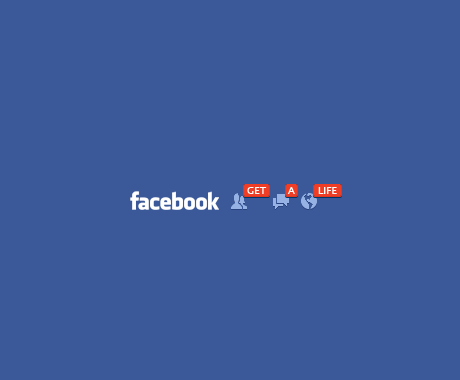
\includegraphics[width=1.00\textwidth]{img/1211-facebook-get-a-life_0.png}~\\
		\emph{<<Get a life>> (va t'acheter une vie), le logo Facebook d{\'e}tourn{\'e} (Boltron/Flickr/CC)~\footnotemark}
		
	\end{center}
\end{minipage} \hfill \begin{minipage}[h]{0.55\textwidth}
	<<Cela faisait un an et demi que j'y pensais>>, <<j'ai eu beaucoup de mal {\`a} sauter le pas>> ... Comme on se pr{\'e}pare {\`a} arr{\^e}ter la cigarette, les internautes que Rue89 a rencontr{\'e}s ont longtemps m{\^u}ri l'id{\'e}e de quitter \texttt{Facebook~\footnotemark}. ~\\

	R{\'e}cemment, ils ont d{\'e}cid{\'e} de rompre avec cette communaut{\'e} de 800 millions de personnes, dont 23 millions d'<<amis>> fran\c{c}ais. ~\\

	Pour Sevin, \texttt{blogueuse~\footnotemark} de 28 ans, le r{\'e}seau social avait perdu de son int{\'e}r{\^e}t. Aussi bien ses statuts, {\'e}crits et publi{\'e}s sur un coup de t{\^e}te et presque aussit{\^o}t effac{\'e}s, que ceux des autres : ~\\
	
	\begin{minipage}[h]{0.10\textwidth} ~\\ \end{minipage} \hfill \begin{minipage}[h]{0.70\textwidth}
		<<Je me d{\'e}solais de voir les contenus tr{\`e}s personnels que mes contacts postaient. Je n'aimais plus cette mani{\`e}re d'interagir avec eux. C'est une consommation d{\'e}bilisante, on bouffe la vie des autres.>>
	\end{minipage} \hfill \begin{minipage}[h]{0.15\textwidth} ~\\ \end{minipage} ~\\~\\	
\end{minipage} ~\\ ~\\
\footnotetext{\texttt{http://www.flickr.com/photos/boltron/4461019149/}}
\footnotetext{\texttt{http://www.rue89.com/facebook}}
\footnotetext{\texttt{http://www.recommande-ar.com/2012/02/02/pourquoi-jai-supprime-mon-compte-facebook/}}

\textbf{<<Si tu n'as pas plus de 300 amis, tu n'es rien>>}~\\

Au coll{\`e}ge ou au lyc{\'e}e, les histoires et les rumeurs naissent sur Facebook. On y r{\`e}gle ses comptes. On y entre en comp{\'e}tition pour le plus grand nombre d'amis ou de <<J'aime>> sous une photo. Manon, 18 ans, raconte : ~\\

\begin{minipage}[h]{0.10\textwidth} ~\\ \end{minipage} \hfill \begin{minipage}[h]{0.70\textwidth}
	<<Ce monde virtuel d{\'e}grade la notion d'amiti{\'e} avec ses chiffres. Si tu n'as pas plus de 300 amis, tu n'es rien, tu n'es pas ``populaire''... combien de fois on nous l'a dit ou fait sentir.>>
\end{minipage} \hfill \begin{minipage}[h]{0.15\textwidth} ~\\ \end{minipage} ~\\~\\

Un petit jeu parfois cruel que Pauline, 15 ans, ne supportait plus : ~\\

\begin{minipage}[h]{0.10\textwidth} ~\\ \end{minipage} \hfill \begin{minipage}[h]{0.70\textwidth}
	<<Facebook m'apportait plus de soucis que de joies. Je l'ai quitt{\'e} parce que j'{\'e}tais dans une p{\'e}riode o{\`u} j'avais besoin de me couper un peu de ce monde superficiel et faux. >>
\end{minipage} \hfill \begin{minipage}[h]{0.15\textwidth} ~\\ \end{minipage} ~\\~\\

\textbf{<<Facebook r{\'e}cup{\`e}re toutes nos donn{\'e}es>>}~\\

Quitter le r{\'e}seau social {\'e}tait d'abord un acte militant pour Antonin Moulart, {\'e}tudiant et membre d'\texttt{Internet sans fronti{\`e}res~\footnotemark}. Sur \texttt{son blog~\footnotemark}, cet activiste du Web encourage les lecteurs {\`a} suivre son exemple : ~\\
\footnotetext{\texttt{http://www.internetsansfrontieres.com/}}
\footnotetext{\texttt{http://antonin.moulart.org/}}

\begin{minipage}[h]{0.10\textwidth} ~\\ \end{minipage} \hfill \begin{minipage}[h]{0.70\textwidth}
	<<Je ne suis pas anti-Facebook mais je vois les d{\'e}rives. C'est un syst{\`e}me h{\'e}g{\'e}monique cot{\'e} en Bourse. Ils font de la publicit{\'e} ultra-cibl{\'e}e, r{\'e}cup{\`e}rent toutes nos donn{\'e}es et notre carnet d'adresses. Ils m{\'e}morisent tout et il est impossible d'y {\'e}chapper. >>
\end{minipage} \hfill \begin{minipage}[h]{0.15\textwidth} ~\\ \end{minipage} ~\\~\\

Une {\'e}tude de \texttt{Lightspeed Research~\footnotemark} montre que 23\% de ceux qui ont r{\'e}duit leur temps de connexion sur Facebook craignaient pour la protection de leurs donn{\'e}es personnelles. ~\\
\footnotetext{\texttt{http://www.lightspeedresearch.com/press-releases/faut-il-craindre-une-baisse-d'activite-sur-les-reseaux-sociaux/}}

\textbf{<<C'est du harc{\`e}lement moral>>}~\\

Selon ces internautes, le r{\'e}seau social devient de plus en plus compliqu{\'e} : les options et la mise en page changent r{\'e}guli{\`e}rement. De plus en plus intrusif : il faut r{\'e}pondre {\`a} deux questions pour simplement retirer son identification d'une photo ind{\'e}sirable. ~\\

Au moment de la suppression du compte, l'internaute doit confirmer, re-confirmer sa d{\'e}marche et m{\^e}me se justifier. Un long processus qui exasp{\`e}re Antonin Moulart : ~\\

\begin{minipage}[h]{0.10\textwidth} ~\\ \end{minipage} \hfill \begin{minipage}[h]{0.70\textwidth}
	<<C'est du harc{\`e}lement moral. Avant la d{\'e}sactivation, on vous dit dans un message ``vous allez manquer {\`a} J{\'e}r{\'e}my, {\`a} Laura, etc.''>>
\end{minipage} \hfill \begin{minipage}[h]{0.15\textwidth} ~\\ \end{minipage} ~\\~\\

Il faut ensuite attendre quatorze jours pour que le compte soit d{\'e}finitivement supprim{\'e}. Un laps de temps qui a mis Sevin, l{\'e}g{\`e}rement d{\'e}pendante et h{\'e}sitante, {\`a} rude {\'e}preuve : ~\\

\begin{minipage}[h]{0.10\textwidth} ~\\ \end{minipage} \hfill \begin{minipage}[h]{0.70\textwidth}
	<<M{\^e}me pour l'avortement, le d{\'e}lai de r{\'e}tractation n'est pas aussi long. Comme s'il n'y avait rien de plus important dans la vie !>>
\end{minipage} \hfill \begin{minipage}[h]{0.15\textwidth} ~\\ \end{minipage} ~\\~\\

\textbf{<<Je vis vraiment mieux sans lui !>>}~\\

Avec le recul, cette d{\'e}sinscription est un soulagement pour Pauline : ~\\

\begin{minipage}[h]{0.10\textwidth} ~\\ \end{minipage} \hfill \begin{minipage}[h]{0.70\textwidth}
	<<Je vis vraiment mieux sans lui !>>
\end{minipage} \hfill \begin{minipage}[h]{0.15\textwidth} ~\\ \end{minipage} ~\\ %% ~\\

Sevin consacre d{\'e}sormais plus de temps {\`a} la lecture, aux sites d'informations... et {\`a} Twitter : ~\\

\begin{minipage}[h]{0.10\textwidth} ~\\ \end{minipage} \hfill \begin{minipage}[h]{0.70\textwidth}
	<<J'ai l'impression d'avoir retrouv{\'e} la vraie vie. >>
\end{minipage} \hfill \begin{minipage}[h]{0.15\textwidth} ~\\ \end{minipage} ~\\ %% ~\\

Mais qu'ils le veuillent ou non, ces ex-utilisateurs de Facebook restent attach{\'e}s au r{\'e}seau social. \texttt{Selon le collectif Europe VS Facebook~\footnotemark}, la soci{\'e}t{\'e} de Mark Zuckerberg conserve les donn{\'e}es personnelles m{\^e}me apr{\`e}s la suppression du compte. ~\\
\footnotetext{\texttt{http://europe-v-facebook.org/FR/Objectifs/objectifs.html}}

Apr{\`e}s une rencontre avec deux repr{\'e}sentants du r{\'e}seau social le 6 f{\'e}vrier {\`a} Vienne, le collectif a cependant annonc{\'e} que \texttt{Facebook s'{\'e}tait engag{\'e} {\`a} changer~\footnotemark} sa proc{\'e}dure pour que <<ces suppressions signifient vraiment suppression>>. ~\\
\footnotetext{\texttt{http://www.europe-v-facebook.org/EN/Media/PR\_1\_en.pdf}}

En attendant, seuls les plus motiv{\'e}s, comme Antonin, feront la d{\'e}marche de r{\'e}clamer ce qui leur appartient {\`a} Mark Zuckerberg. M{\^e}me s'il n'a aucune nouvelle du groupe depuis sa demande, il y a un mois : ~\\

\begin{minipage}[h]{0.10\textwidth} ~\\ \end{minipage} \hfill \begin{minipage}[h]{0.70\textwidth}
	<<J'ai envoy{\'e} un deuxi{\`e}me courrier avec recommand{\'e} pour r{\'e}cup{\'e}rer mes archives compl{\`e}tes. Sinon, je passerai devant la justice.>>
\end{minipage} \hfill \begin{minipage}[h]{0.15\textwidth} ~\\ \end{minipage} ~\\~\\

Selon l'{\'e}tude de Lightspeed Research, 10,5\% des internautes fran\c{c}ais ont <<compl{\`e}tement cess{\'e} d'utiliser>> les r{\'e}seaux sociaux. Ils restent minoritaires. Au cours des six derniers mois, SocialBakers a enregistr{\'e} \texttt{plus d'un million utilisateurs de Facebook suppl{\'e}mentaires~\footnotemark} dans l'Hexagone. ~\\
\footnotetext{\texttt{http://www.socialbakers.com/facebook-statistics/france/last-3-months\#chart-intervals}}

Sur les trois derniers mois, le nombre d'utilisateurs du r{\'e}seau social a baiss{\'e} dans 23 pays dont les Etats-Unis, le Royaume-Uni, Monaco et Hong-Kong. ~\\

\textbf{Le mode d'emploi pour quitter Facebook}~\\

Il est plus facile de dire que l'on va quitter Facebook que de le faire. Rue89 vous explique, {\'e}tape par {\'e}tape, comment proc{\'e}der. ~\\

Il existe deux mani{\`e}res de prendre ses distances avec le r{\'e}seau social. ~\\

\textbf{1 D{\'e}sactiver son compte}~\\

Les informations publi{\'e}es sur votre profil Facebook ne seront plus accessibles mais resteront sur les serveurs du r{\'e}seau social. Si vous changez d'avis, vous pourrez r{\'e}activer votre compte plus tard. ~\\

\begin{itemize}
	\item[$\bullet$] Sur votre page Facebook, cliquez sur la fl{\`e}che en haut {\`a} droite, {\`a} c{\^o}t{\'e} de l'onglet <<Accueil>> ;
	\item[$\bullet$] Choisissez <<Param{\`e}tres du compte>> ;
	\item[$\bullet$] Dans la liste {\`a} gauche, cliquez sur <<S{\'e}curit{\'e}>> puis <<D{\'e}sactiver le compte>> ;
	\item[$\bullet$] Facebook vous demande quelle est la raison de votre d{\'e}part. Cochez la proposition qui correspond (ex : <<Je ne me sens pas en s{\'e}curit{\'e} sur Facebook>>, <<Mon compte a {\'e}t{\'e} pirat{\'e}>>, <<Je ne trouve pas Facebook utile>>, etc.) ;
	\item[$\bullet$] Cliquez sur <<Confirmer>>. Votre compte est maintenant d{\'e}sactiv{\'e}.
\end{itemize}~\\

\textbf{2 Supprimer son compte}~\\

Pas de retour en arri{\`e}re possible. Votre profil sera effac{\'e} d{\'e}finitivement. ~\\

\begin{itemize}
	\item[$\bullet$] Sur votre page Facebook, cliquez sur la fl{\`e}che en haut {\`a} droite, {\`a} c{\^o}t{\'e} de l'onglet <<Accueil>> ;
	\item[$\bullet$] Choisissez <<Aide>> ;
	\item[$\bullet$] Tapez <<Supprimer>> dans le champ de recherche ;
	\item[$\bullet$] S{\'e}lectionnez <<Comment supprimer d{\'e}finitivement mon compte>> dans les r{\'e}sultats propos{\'e}s ;
	\item[$\bullet$] Un texte s'affiche. Dans le troisi{\`e}me paragraphe, cliquez sur le lien <<Faites la demande de suppression ici>> ;
	\item[$\bullet$] Une autre page s'ouvre. Cliquez sur <<Supprimer mon compte>> ;
	\item[$\bullet$] Entrez votre mot de passe et fa{\^i}tes le contr{\^o}le de s{\'e}curit{\'e} (recopiez le texte qui appara{\^i}t dans l'encadr{\'e}).
\end{itemize}~\\

C'est fait ! Votre compte sera supprim{\'e} dans quatorze jours... si vous ne vous reconnectez pas entre temps. ~\\

\end{document}